%
%
%
%
\section{Introduction}
\headb{Transonic Turbine Stage}{Introduction}
\label{rt27_introduction.sec}
%
 Two different numerical techniques
 for the calculation of steady and unsteady aerodynamics have been
 presented in the previous two chapter.
 These two methods will now be used for the investigation
 of the unsteady pressure fluctuations on a typical rotor blade.
 The unsteadiness is caused
 by its relative motion with respect the upstream stationary
 nozzle guide vane (NGV).
 The data required for such an investigation consists only of
 the two blade geometries, the stationary flow boundary
 conditions upstream of the NGV blade and downstream of the rotor blade and
 the rotational speed.
 The analysis process begins with the calculation
 of the steady-state flow-field for the given set of flow conditions
 and rotational speed.
 The next step is the evaluation of the unsteady rotor pressure
 fluctuations caused by both wake and potential effects.
 A description of the unsteady phenomena of interest, unsteady pressure
 fluctuations on the rotor blade, will be given in some detail.
 The the details of the experimental work carried out at Oxford
 Osney Laboratory will also be included for the sake
 of completeness.
%
%
%
\subsection{Description of the problem}
\label{rt27_description.sec}
%
 The first step towards the unsteady aerodynamics
 analysis of turbomachinery blades, is the computation
 of the corresponding steady non-linear flow.
 A multistage steady-state flow will be presented in section \ref{rt27_steady.subsec}
 and its complex features such secondary flows, tip-leakage losses
 will be discussed in some details.

 Once the steady-state flow is known the question is the selection
 of a ``best analysis'' for the prediction of unsteady effects.
 Before offering an answer to this, it is appropriate to discuss, first,
 what one would hope to get out of such calculations. The focus of this
 chapter is a numerical tool that can be used by
 designers as a part of an industrial design system.
 Major concernsdue to flow unsteadiness are the possibility
 of blade flutter and excessive forced response.
 Flutter is by definition a linear problem since it is concerned with
 possible growth of infinitesimal unsteady perturbations.
 A growing body of evidence suggests that the forced response problem is
 also largely linear. Comparison between linear and non-linear calculations,
 for levels of unsteadiness typical of engine conditions, show that the linear
 calculations predict the forced response to within $5\%$
 (Hall \citeyearNP{Hall:4}, Suddhoo et al. \citeyearNP{Giles:12}).
 This level of accuracy is perfectly adequate for all practical engineering
 design purposes and is probably within the level of other modelling errors.

 For these reasons an unsteady linear Navier-Stokes analysis is performed
 on the rotor blade in order to evaluate the magnitude of unsteady loads
 caused by its relative motion with respect the upstream nozzle guide vane.
 Such a route offers great advantages over non-linear time marching methods
 in terms of speed and storage, while still retaining the key features of
 the flow.

 The sources of unsteadiness are evaluated from the NGV outlet non-uniformities
 and imposed as boundary conditions at the inlet of the rotor passage.
 More specificly the NGV outlet non-uniformities are Fourier decomposed and
 split into vortical and potential components. Each Fourier mode
 is associated with its own unsteady frequency and interblade-phase angle as described
 in appendix \ref{waves.chap}.
 Two linear calculations are performed for each Fourier mode: the vortical-rotor
 interaction, also labelled wake-rotor interaction, and the potential flow interaction.
 Following this route it is possible to estimate the relative influence of
 the NGV wake and potential flow field on the rotor unsteady aerodynamics.
 Since the governing equation are linears the two unsteady solutions can be superimposed
 to give the total unsteady loads for a given Fourier mode.
 This approach is relatively straightforward as well as beeing a suitable tool for
 an industrial design system.
%
\begin{table}[h]
\vspace{5mm}
\begin{center}
\begin{tabular}{|l|l|}\hline\hline
 Number of NGV blades & 36\\ \hline
 Number of rotor blades & 60\\ \hline
 Rotor tip diameter & 554 mm \\ \hline
 Rotor tip clearance & 0.5 mm \\ \hline
 NGV-rotor spacing & 0.346 NGV axial chord \\ \hline
 Design speed & 8434 RPM \\ \hline
 NGV inlet total pressure $p\sm{01}$ & 804505 Pa \\ \hline
 NGV inlet total temperature $T\sm{01}$ & 374.4 K \\ \hline
 NGV outlet isentropic Mach number $M\sm{2is}$ & 0.96 \\ \hline
\hline
\end{tabular}
\end{center}
\caption{Stage characteristics of Rig RT27a}
\label{rt27.tab}
\end{table}
%

 The turbine stage used for this investigation is the well-known
 benchmark Rig RT27a of the Oxford Osney Laboratory. This
 turbine stage represents a typical HP stage of contemporary
 turbomachines and its characteristics are summarised in table \ref{rt27.tab}.
 The computed results are compared with measured Rig RT27a data
 in order to achieve a better understanding of the unsteady effects and
 to assess the applicability bounds of the linear methods for the
 analysis of unsteady 3D NGV-rotor interaction.
%
%
%
%
\subsection{Experimental details}
\label{rt27_experiment.subsec}
%
 Rig RT27a was designed to provide steady and unsteady flow data for typical
 turbine blade geometries at representative engine conditions.
 The turbine stage was mounted in a transient flow turbine test facility
 based on an isentropic light piston tunnel at the Osney laboratory, Oxford
 (Moss et al. \citeyearNP{Moss:1}).
 The rotor blade is a transonic shroudless design of 0.5 m tip diameter with
 an NGV-rotor spacing of 0.346 NGV axial chord.
 Fig. \ref{stage1.fig} shows a meridional view of the stator-rotor
 configuration. The rotor blade presents an evident tip clearance
 which has been set to 0.05 cm ($\approx 1\%$ of rotor span).
%
%
\begin{figure}[ht]
   \centerline{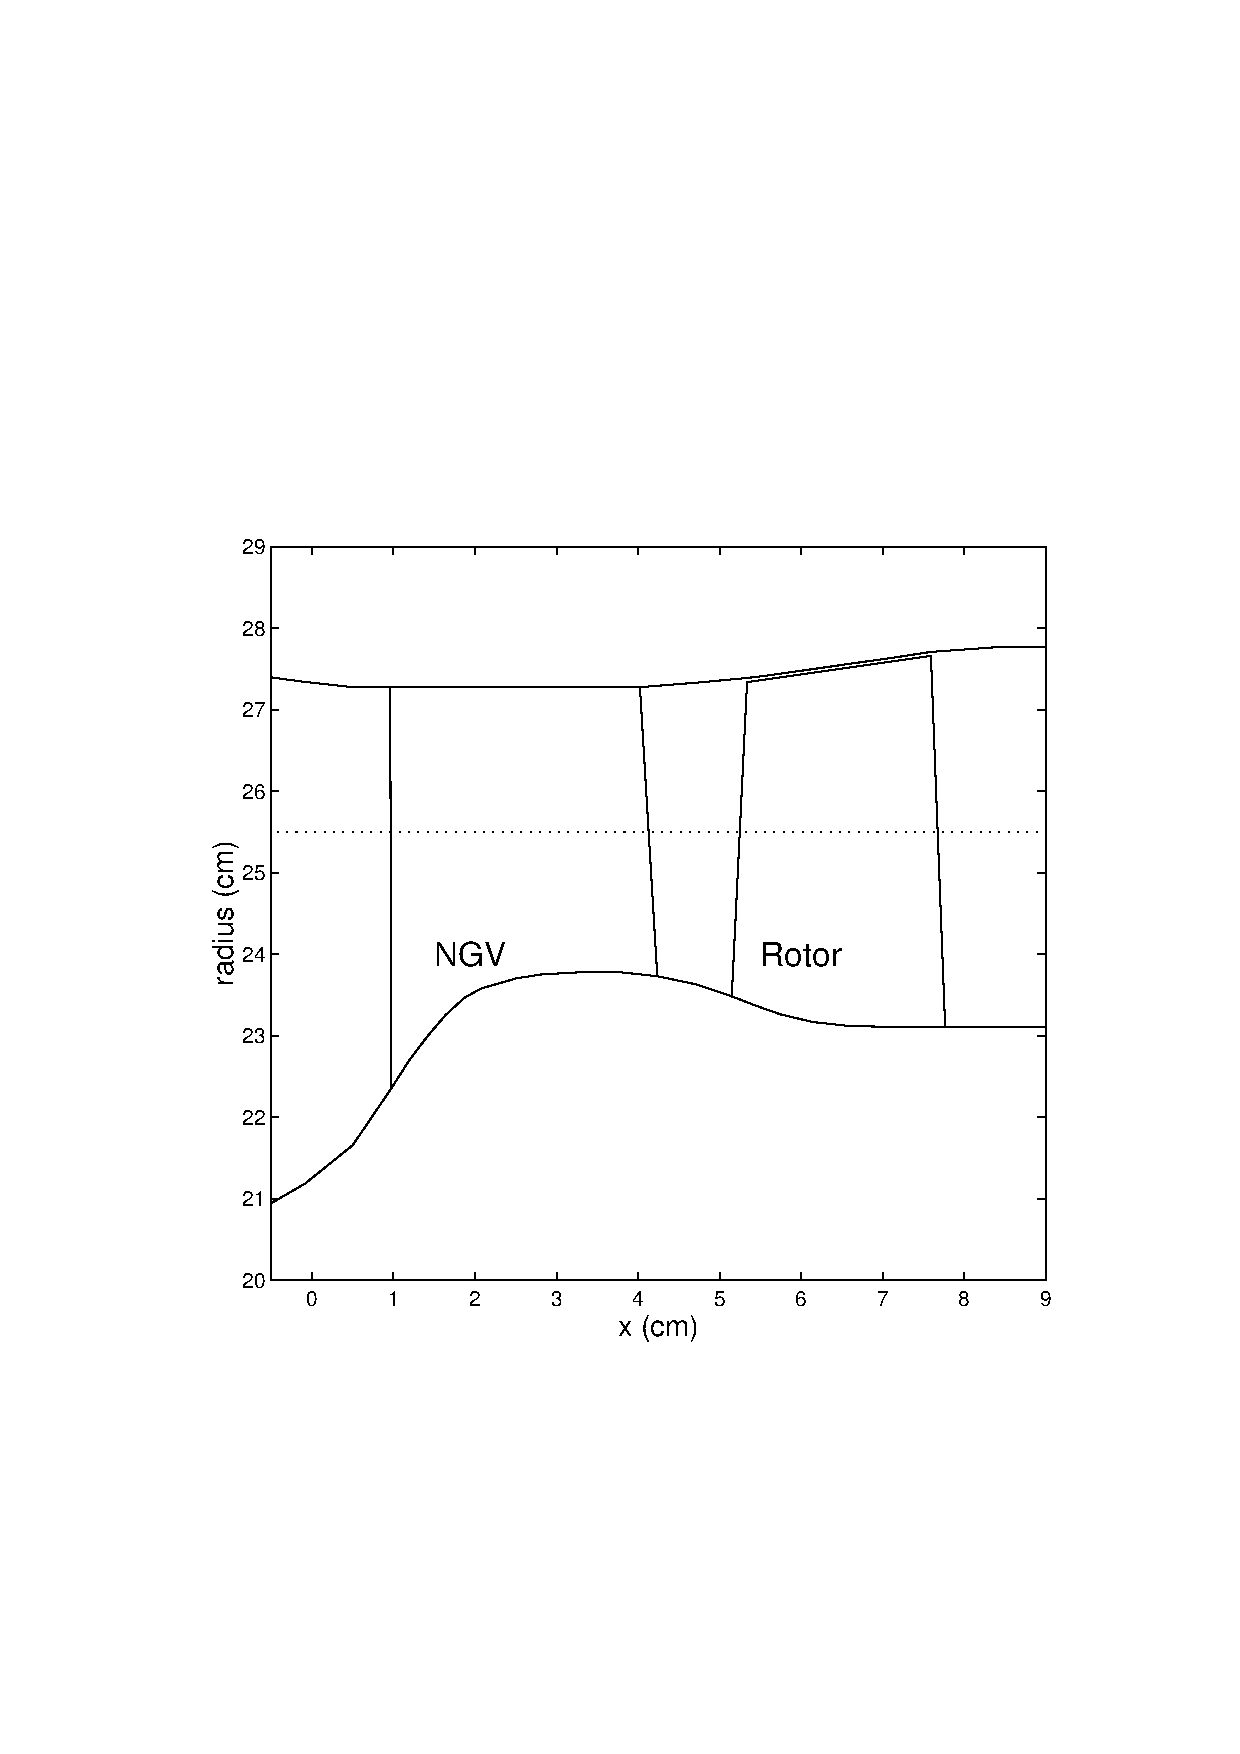
\includegraphics[width=100mm,clip=t]{CHAP_RT27/FIGURE/stage1.pdf}}
   \caption{Meridional view of the RT27a turbine stage}
   \label{stage1.fig}
\end{figure}
%
 The rotor instrumentation, described by Moss et al. \citeyear{Moss:1}, consists
 of 78 flush-mounted miniature pressure transducers, ``surface kulites'',
 and 12 ``leading-edge'' pitot transducers. The latter are protruded from the leading-edge
 with a small bell-mouth to reduce sensitivity to incidence changes.
 The kulite transducers are arranged at span-wise
 positions of 5, 10, 50, 90 and $95\%$ of annulus height;
 these sections will be referred to as root, mid-root, mid-height, mid-tip and
 top.

 Prior to a run, the rotor is accelerated to 6000 RPM, in vacuum,
 by an air motor.
 Once this rotational speed is reached, a fast-acting annular valve
 opens and the air (at suitable temperature and pressure
 generated by a free-sliding piston in the pump tube) passes
 through the turbine stage for a duration of 200 ms. The rotor accelerates
 to 9500 RPM and the data are recorded
 for some 17 ms while the rotor passes through the design condition.
 Since the blade passing frequency is approximately 5 kHz,
 the 17 ms acquisition time is sufficient to capture 85
 wake passing cycles.
 The experimental data presented by by Moss et al. \citeyear{Moss:1},
 have been assembled from over 400 signals
 captured during 120 tunnel runs. The tolerance on the pressure measurements
 is $\pm 1.75 \%$ with a $95\%$ confidence limit.
 This is equivalent to a Mach number accuracy of $\pm 0.02$
 at a Mach number of 0.65.
%
